\documentclass[conference]{IEEEtran}
\IEEEoverridecommandlockouts
% The preceding line is only needed to identify funding in the first footnote. If that is unneeded, please comment it out.
\usepackage{cite}
\usepackage{amsmath,amssymb,amsfonts}
\usepackage{algorithmic}
\usepackage[ruled,noline,linesnumbered,noend]{algorithm2e}
\usepackage{graphicx}
\usepackage{textcomp}
\usepackage{xcolor}
\usepackage{pgfplots}
%\pgfplotsset{width=10cm,compat=1.9}

% algorithm styling
\SetInd{0.5em}{0.2em}       % reduce indent
\newcommand\mycommentfont[1]{\footnotesize\sffamily{#1}}
\SetCommentSty{mycommentfont}

% fun with colors
\RequirePackage{color}
\usepackage{colortbl}
\definecolor{RED}{rgb}{1,0,0}
\definecolor{BLUE}{rgb}{0,0,1}
\definecolor{GREEN}{rgb}{0,1,0}
\definecolor{color1}{rgb}{0.913, 0.776, 0.686}
\definecolor{color2}{rgb}{0.913, 0.867, 0.686}
\definecolor{ltgray}{rgb}{0.85, 0.85, 0.85}

% notes, remarks, todo
\newcommand{\Remark}[1]{{\color{RED}\sf Remark: {#1}}}
\newcommand{\tp}[1]{{\color{RED}\sf TP: {#1}}}
\newcommand{\dm}[1]{{\color{BLUE}\sf DM: {#1}}}
\newcommand{\Fix}[1]            {\textcolor{red}{\small\sf [#1]}}
\newcommand{\kw}[1]             {{\tt #1}\xspace}
\newcommand{\todo}[1]{
      \addcontentsline{tdo}{todo}{\protect{#1}}
      \marginpar{\colorbox{white!90!black}{\textcolor{red}{
      \parbox{2.1cm}{\scriptsize\bf\raggedright #1}
      }}}
}

\usepackage{etoolbox}

\def\BibTeX{{\rm B\kern-.05em{\sc i\kern-.025em b}\kern-.08em
    T\kern-.1667em\lower.7ex\hbox{E}\kern-.125emX}}
\begin{document}

\title{Parallel Domain Decomposition Techniques Applied to Multi-Variate Functional Approximation of Discrete Data\\
%{\footnotesize \textsuperscript{*}Note: Sub-titles are not captured in Xplore and should not be used}
%\thanks{Identify applicable funding agency here. If none, delete this.}
\thanks{Early Career Research Program, Department of Energy, US}
}


\author{\IEEEauthorblockN{1\textsuperscript{st} Vijay S. Mahadevan}
\IEEEauthorblockA{\textit{Mathematics and Computational Science Division} \\
\textit{Argonne National Laboratory}\\
Lemont, IL, 60439, USA \\
mahadevan@anl.gov}
\and
\IEEEauthorblockN{2\textsuperscript{nd} Thomas Peterka}
\IEEEauthorblockA{\textit{Mathematics and Computational Science Division} \\
\textit{Argonne National Laboratory}\\
Lemont, IL, 60439, USA \\
tpeterka@mcs.anl.gov}
\and
\IEEEauthorblockN{3\textsuperscript{rd} Iulian Grindeanu}
\IEEEauthorblockA{\textit{Mathematics and Computational Science Division} \\
\textit{Argonne National Laboratory}\\
Lemont, IL, 60439, USA \\
iulian@anl.gov}
\and
\IEEEauthorblockN{4\textsuperscript{th} Youssef Nashed}
\IEEEauthorblockA{\textit{Stats Perform}\\
Chicago, IL, 60601, USA \\
youssef.nashed@statsperform.com}
}

\maketitle

\begin{abstract}
Compactly expressing large-scale datasets through multivariate functional approximations (MFA) can be critically important for analysis and visualization to drive scientific discovery. This paper presents a data and domain partitioning approach to scalably compute a MFA representation, by reducing the total work per task in combination with a nonlinear Schwarz-type, inner-outer iterative scheme for converging the interface data. For the underlying MFA, we utilize a tensorial expansion of non-uniform B-spline (NURBS) basis to adaptively reduce the functional approximation error in the input data. While previous work on adaptive NURBS-based MFA has been proven successful, the computational complexity for encoding large datasets on a single process can be prohibitive. We demonstrate effectiveness of the presented approach with an overlapping Jacobi-Schwarz based domain decomposition solver, with a nonlinear accelerator such as L-BFGS or Krylov (nCG, L-GMRes) to minimize the subdomain error residuals obtained from decoding the MFA, and more specifically to resolve the discontinuities at boundaries. The analysis of the presented scheme for some analytical and real scientific datasets in 1-D and 2-D are also presented. Additionally, scalability studies are also shown for some real-world 2-d datasets to evaluate the parallel speedup of the algorithm on large clusters.
\end{abstract}

\begin{IEEEkeywords}
functional approximation, domain decomposition, scalable methods
\end{IEEEkeywords}

\section{Introduction}

Large scale discrete data analysis from various scientific computational simulations often require high-order continuous functional representations that have to be evaluated anywhere in the domain. Such expansions described as Multivariate Functional Approximations (MFA) in arbitrary dimensions \cite{nurbs-book} allow the original discrete data to be compressed, and expressed in a compact closed form in addition to supporting higher-order derivative queries. One particular option is to use NURBS bases for the MFA encoding of scattered data \cite{peterka-mfa}. Due to the potentially large datasets that need to be encoded into a MFA, the need for computationally efficient algorithms (in both time and memory) to partition the work into subtasks is critically important. 

In the current paper, we utilize domain decomposition (DD) techniques \cite{smith-ddm} with data partitioning strategies to produce scalable algorithms to adaptively compute the MFA to reproduce a given dataset within user-specified tolerances. In such partitions, it is imperative to ensure that the continuity of the data across subdomain interfaces are maintained and is consistent with the degree of the underlying bases used in the MFA. 
We present an iterative DD scheme with an outer Schwarz-type iterative scheme in order to ensure that continuity is recovered, and the overall error stays bounded when number of subdomains are increased (subdomain size decreases).

%{\color{red}THIS IS A DRAFT}

%\begin{itemize}
%	\item Talk about MFA and how it can be used to approximation discrete solution data. Reference previous work.
%	\item Provide motivations on why this is necessary especially for large datasets
%	\item Literature survey of other work for parallel interpolation and compression of data
%	\item What are the other approaches to address this issue; pros and cons
%\end{itemize}

The paper is organized as follows. Section 2 summarizes the related work in using variations of the Schwarz scheme for scalably interpolating data, and using constraints for recovering continuity along discontinuous patches. Section 3 provides details about the constrained optimization problem to resolve subdomain boundary discontinuities, along with the outer-inner DD based solver setup to compute the continuous MFA. Next the application of the DD solver for 1-D/2-D analytical problems are provided to verify error convergence, and scalability of the hierarchical scheme with decreasing subdomain size under overlap specifications. Finally, the parallel scalability of the scheme is presented for some real-world cases to adaptively compute the MFA within user-specified tolerances.


\section{Related Work}

DD techniques for parallel interpolation of scattered data has been explored previously with Radial Basis Functions (RBF) \cite{mai-approx-rbf}, yielding good scalability to create a MFA that closely replicates underlying profile. Additionally, use of restricted Additive-Schwarz preconditioners with GMRes iterative solvers have been shown to be scalable \cite{yokota-rasm-rbf} for such problems. However, using NURBS-basis to compute MFA in parallel, while maintaining higher-order continuity across subdomains has not been explored previously in this context. To overcome the issues with discontinuities along NURBS patches, \cite{zhang-nurbs-continuity} have proposed to use a gradient projection scheme to constrain the value (G0), the gradient (G1) and the hessian (G2) at a small number of test points for optimal shape recovery. 


While it is also possible to create such a constrained recovery during the actual post-processing stage i.e., decoding of the MFA through blending techniques \cite{grindeanu-blending}, the underlying MFA representation would remain discontinuous, and would become more so with increasing number of subdomains. In contrast, we propose an extension to the constrained solvers used by \cite{zhang-nurbs-continuity, xu-jahn-discrete-adjoint} by utilizing a recursive DD-based parallel outer-inner iterative scheme to resolve continuity prescriptions as required by the user. The outer iteration utilizes a flavor of the restricted Additive-Schwarz method (RASM) \cite{gander-rasm}, Jacobi-Schwarz \cite{smith-ddm}, with an efficient, inner subdomain solver using L-BFGS as used in \cite{zheng-bo-bspline-bfgs}, or Krylov-type schemes to minimize the decoded residual within acceptable error tolerances. This DD solver has low memory requirements that scales with growing subdomains, and only imposes nearest neighbor communication of the interface data once per outer iteration. 

** talk about nearest neighbor communication is done once per outer iteration; better than say multiplicative schwarz even if convergence is slightly slower; 

** think about MFA refs and DIY ?

** PetIGA and other parallel NURBS algos/software

\section{Approach}

Domain decomposition techniques in general rely on the idea of splitting a larger domain into smaller subdomains that are coupled through an interface layer. Typical applications in Boundary-Value problems (BVP) \cite{smith-ddm} have been employed successfully for efficiently computing the solution to large Partial Differential Equations (PDEs) and the approach employed in the current work is to utilize such schemes to compute consistent and accurate MFA representations in parallel. Similar to DD for PDE applications, the amount of overlap in the data for MFA controls the convergence speed and scalability of the overall algorithm.

For illustration, consider a 1-D domain with two partitions as shown in Fig. \ref{fig:DD-subdomain-illiustration}.

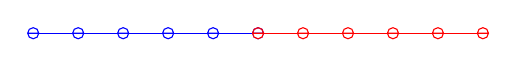
\begin{tikzpicture}
\begin{axis}[cycle list name=exotic, legend style={draw=none}, axis lines=none, xtick=\empty, ytick=\empty]
%\addplot coordinates {(0,1) (0.1,1) (0.2,1) (0.3,1) (0.4,1) (0.5,1) (0.6,1) (0.7,1) (0.8,1) (0.9,1) (1,1)};
\addplot[domain=0:0.5, samples=6, color=blue, mark=halfcircle] {1};
\addplot[domain=0.5:1, samples=6, color=red, mark=halfcircle] {1};
\end{axis}
\label{fig:DD-subdomain-illiustration}
\end{tikzpicture}


\begin{itemize}
	\item What are we proposing and why this can be a stable technique to recover high-order continuity in parallel ?
	\item Give context about DD methods and how ASM in this context makes sense 
	\item Refer to \cite{smith-ddm} and \cite{ddm-rbf-fast} as well and write out the equations with \cite{nurbs-book} help
\end{itemize}

\subsection{Methodology}

Explain the iterative scheme in terms of the underlying equations and how the boundary terms are resolved through a global ASM method. First start with 1-d and talk about extensions in the scheme to allow arbitrary dimensional solver framework.

\begin{eqnarray} \label{asm}
L_1U^{n}_1=f_1(x) \in \Omega_1  \\
L_1U^{n}_1=g(x) \in \partial\Omega_1 \\ 
U^{n}_1 = U^{n-1}_2 \in \partial\Omega_1 \\
L_2U^{n}_2=f_2(x) \in \Omega_2 \\
L_2U^{n}_2=g(x) \in \partial\Omega_2 \\
U^{n}_2 = U^{n-1}_1 \in \partial\Omega_2
\end{eqnarray}


\subsection{Implementation}

Talk about DIY and Python implementations for the code. Provide algorithmic references here as well.

We implemented the code in this article in Python using pyDIY. DIY~\cite{morozov16} is a programming model and runtime
for block-parallel analytics on distributed-memory machines, built on MPI-3~\cite{dongarra13}.  Rather than programming
for process parallelism directly in MPI, the programming model in DIY is based on block parallelism: data are decomposed
into subdomains called blocks; blocks are assigned to processing elements (processes or threads); computation is
described over these blocks, and communication between blocks is defined by reusable patterns. The same DIY program
consisting of a block-parallel decomposition can be run on different numbers of MPI processes: it is the job of the DIY
runtime to map between blocks and processes. A recent development in DIY is a development branch of pyDIY~\cite{pydiy},
a set of Python bindings for DIY, using pybind11~\cite{jakob17} and mpi4py~\cite{dalcin11}.

The overall approach is sketched in Algorithm~\ref{alg:pseudocode}. \Remark{Vijay: finish the pseudocode and expand the
discussion of it below.} We begin by decomposing the domain into a set of regular blocks aligned with the principal axes
of the global domain. We then begin iterating over the blocks in a 2-level nested loop: the outer loop is the ASM
approach described above, while the inner loop is a nonlinear optimization (BFGS or Krylov) to solve for the control
points of the MFA model in each block. At the bottom of each ASM iteration, we exchange the constraints
among neighboring blocks in a regular nearest-neighbor communication pattern, and we also perform a global
collective communication to determine whether the solution has converged to the desired error tolerance.

\Remark{Algorithm~\ref{alg:pseudocode} is just a skeleton. Details need to be filled in. Termination conditions, local
(inner loop) iterative scheme, types of constraints (control points or decoded points), etc.}

\begin{algorithm}
    \DontPrintSemicolon
    decompose domain into blocks\;
    \tcp*[h]{Outer ASM loop}\;
    \While{not globally done}
    {
        constraints $\leftarrow$ dequeue incoming constraints\;
        \tcp*[h]{Inner BFGS or Krylov optimization loop}\;
        \While{error decreasing and $iterate < max\_iterations$}
        {
            solve local MFA\;
            enqueue constraints to neighbor blocks\;
        }
        exchange constraints with neighbor blocks\;
        collect global error\;
    }
    \caption{\Remark{Caption TBD}}
    \label{alg:pseudocode}
\end{algorithm}


\section{Results}

Explain about the common problem datasets that we are going to be using and why they have been chosen.

Please note sections \ref{AA}--\ref{SCM} below for more information on 
proofreading, spelling and grammar.

\subsection{1-d Results}\label{AA}

Problem setups
\begin{itemize}
  \item Sine
  \item Sinc
  \item S3D
  \item Nuclear data
\end{itemize}

\begin{itemize}
	\item Use the first two problems to measure convergence in parallel as number of domains increase
	\item Talk about adaptivity and resolution of data even for highly varying problem data.
\end{itemize}

\subsection{2-d Results}

Problem setups
\begin{itemize}
	\item Sinc
	\item Nek5000
	\item S3D
\end{itemize}


\begin{itemize}
	\item Adaptive algorithms to resolve data and provide compression
	\item DD scheme with ASM in combination with adaptivity.
	\item Discuss about complications and potential ways to enforce continuity. (a) Use decoded data, (b) Use control point space across interface
\end{itemize}

\subsection{Parallel Scalability}

Showcase some scalability results on Bebop for the 2-d problem; Take S3D and CESM datasets, along with artificial sinc combination functions.

How does the nearest neighbor communication stay bounded ?

%\paragraph{Positioning Figures and Tables} Place figures and tables at the top and 
%``Fig.~\ref{fig}'', even at the beginning of a sentence.

%\begin{table}[htbp]
%\caption{Table Type Styles}
%\begin{center}
%\begin{tabular}{|c|c|c|c|}
%\hline
%\textbf{Table}&\multicolumn{3}{|c|}{\textbf{Table Column Head}} \\
%\cline{2-4} 
%\textbf{Head} & \textbf{\textit{Table column subhead}}& \textbf{\textit{Subhead}}& \textbf{\textit{Subhead}} \\
%\hline
%copy& More table copy$^{\mathrm{a}}$& &  \\
%\hline
%\multicolumn{4}{l}{$^{\mathrm{a}}$Sample of a Table footnote.}
%\end{tabular}
%\label{tab1}
%\end{center}
%\end{table}

%\begin{figure}[htbp]
%\centerline{\includegraphics{fig1.png}}
%\caption{Example of a figure caption.}
%\label{fig}
%\end{figure}

\section{Conclusion}

\begin{itemize}
	\item What did we implement to enhance speedup of the MFA framework and did we preserve accuracy of the underlying method ?
	\item Did we speedup the actual computation by performing DD with ASM global iterations for some of the problem data ?
	\item Does the method scale as a function of domains and problem size ? 
	\item What advantages does it provide for fix-up schemes that can be used in a post-processing step (ref Iulian's blending idea) ?
	\item Future extensions to T-splines and local adaptivity and potential complications involved
\end{itemize}

\section*{Acknowledgment}

This work is supported by Advanced Scientific Computing Research, Office of Science, U.S. Department of Energy, under
Contract DE-AC02-06CH11357, program manager Laura Biven. We gratefully acknowledge the computing resources provided on
Bebop, a high-performance computing cluster operated by the Laboratory Computing Resource Center (LCRC) at Argonne
National Laboratory.

\Remark{Inconsistent bib styles. Should really be using the same method throughout, either bibtex or thebibliography.}

\AtEndEnvironment{thebibliography}{
% \begin{thebibliography}{00}

\bibitem{nurbs-book} Piegl, Les, and Wayne Tiller. The NURBS book. Springer Science \& Business Media, 2012.

\bibitem{peterka-mfa} Peterka, Tom, S. G. Youssef, Iulian Grindeanu, Vijay S. Mahadevan, Raine Yeh, and Xavier Tricoche. "Foundations of multivariate functional approximation for scientific data." In 2018 IEEE 8th Symposium on Large Data Analysis and Visualization (LDAV), pp. 61-71. 2018.

\bibitem{nashed-rational} Nashed, Youssef SG, Tom Peterka, Vijay Mahadevan, and Iulian Grindeanu. "Rational Approximation of Scientific Data." In International Conference on Computational Science, pp. 18-31. Springer, Cham, 2019.

\bibitem{grindeanu-blending} Grindeanu, Iulian, Tom Peterka, Vijay S. Mahadevan, and Youssef SG Nashed. "Scalable, High-Order Continuity Across Block Boundaries of Functional Approximations Computed in Parallel." In 2019 IEEE International Conference on Cluster Computing (CLUSTER), pp. 1-9. IEEE, 2019.

%\bibitem{raine-knot-placement} Yeh, R., Nashed, Y., Peterka, T., Tricoche, X.: Fast Automatic Knot Placement Method for Accurate B-spline Curve Fitting. Submitted to Journal of Computer-Aided Design, 2020.

\bibitem{zheng-bo-bspline-bfgs} Zheng, Wenni, Pengbo Bo, Yang Liu, and Wenping Wang. "Fast B-spline curve fitting by L-BFGS." Computer Aided Geometric Design 29, no. 7 (2012): 448-462.

\bibitem{mai-approx-rbf} Mai-Duy, Nam, and Thanh Tran-Cong. "Approximation of function and its derivatives using radial basis function networks." Applied Mathematical Modelling 27, no. 3 (2003): 197-220.

\bibitem{yokota-rasm-rbf} Yokota, Rio, Lorena A. Barba, and Matthew G. Knepley. "PetRBF—A parallel O (N) algorithm for radial basis function interpolation with Gaussians." Computer Methods in Applied Mechanics and Engineering 199, no. 25-28 (2010): 1793-1804.

\bibitem{smith-ddm} Smith, Barry, Petter Bjorstad, and William Gropp. Domain decomposition: parallel multilevel methods for elliptic partial differential equations. Cambridge university press, 2004.

\bibitem{ddm-rbf} Li, Jichun, and Y. C. Hon. "Domain decomposition for radial basis meshless methods." Numerical Methods for Partial Differential Equations: An International Journal 20, no. 3 (2004): 450-462.

\bibitem{ddm-rbf-fast} Beatson, Richard K., W. A. Light, and S. Billings. "Fast solution of the radial basis function interpolation equations: Domain decomposition methods." SIAM Journal on Scientific Computing 22, no. 5 (2001): 1717-1740.

\bibitem{xu-jahn-discrete-adjoint} Xu, Shenren, Wolfram Jahn, and Jens‐Dominik Müller. "CAD‐based shape optimisation with CFD using a discrete adjoint." International Journal for Numerical Methods in Fluids 74, no. 3 (2014): 153-168.

\bibitem{zhang-nurbs-continuity} Zhang, Xingchen, Yang Wang, Mateusz Gugala, and Jens-Dominik Müller. "Geometric continuity constraints for adjacent NURBS patches in shape optimisation." In ECCOMAS Congress, vol. 2, p. 9316. 2016.

\bibitem{lions-asm} Lions, Pierre-Louis. "On the Schwarz alternating method. I." In First international symposium on domain decomposition methods for partial differential equations, vol. 1, p. 42. 1988.

\bibitem{gander-rasm} Efstathiou, Evridiki, and Martin J. Gander. "Why restricted additive Schwarz converges faster than additive Schwarz." BIT Numerical Mathematics 43, no. 5 (2003): 945-959.

}
% \end{thebibliography}

\bibliographystyle{IEEEtran}
\bibliography{tom}

%\vspace{12pt}
%\color{red}
%IEEE conference templates contain guidance text for composing and formatting conference papers. Please ensure that all template text is removed from your conference paper prior to submission to the conference. Failure to remove the template text from your paper may result in your paper not being published.

\end{document}
